% Created 2025-04-29 Tue 19:26
% Intended LaTeX compiler: pdflatex
\documentclass[11pt]{article}
\usepackage[utf8]{inputenc}
\usepackage[T1]{fontenc}
\usepackage{graphicx}
\usepackage{longtable}
\usepackage{wrapfig}
\usepackage{rotating}
\usepackage[normalem]{ulem}
\usepackage{amsmath}
\usepackage{amssymb}
\usepackage{capt-of}
\usepackage{hyperref}
\usepackage{minted}
\usepackage{siunitx}
\author{Hankertrix}
\date{\today}
\title{Metabolism Notes}
\hypersetup{
 pdfauthor={Hankertrix},
 pdftitle={Metabolism Notes},
 pdfkeywords={},
 pdfsubject={},
 pdfcreator={Emacs 30.1 (Org mode 9.7.11)}, 
 pdflang={English}}
\begin{document}

\maketitle
\setcounter{tocdepth}{2}
\tableofcontents \clearpage\newpage
\section{Definitions}
\label{sec:org918b136}

\subsection{Energy}
\label{sec:org15d9347}
Energy is the ability to do work.
\subsection{Kinetic energy}
\label{sec:org4411607}
Kinetic energy is a form of energy associated with the motion of objects. Examples of kinetic energy include:
\begin{itemize}
\item A cheetah running
\item A hummingbird vibrating its wings
\item A bacterium swimming
\item Blood flowing inside the veins
\end{itemize}
\subsection{Heat energy}
\label{sec:org57aa6e5}
Heat or thermal energy is generated by the random movement of atoms or molecules. In living systems, metabolic activities generate heat. Accumulation of this heat may often require mechanisms to dissipate (through homeostasis), like by sweating or panting in order to maintain the normal body temperature.
\subsection{Electrical energy}
\label{sec:org62f222f}
Electrical energy is manifested in different ways in biological systems. Some examples include electrical impulses in neurons and electrical currents on the surface of electric eels.
\subsection{Light energy}
\label{sec:org72d71c2}
Light energy can be captured by living systems such as during photosynthesis and transformed to other forms such as chemical energy stored in ATP and glucose. Some organisms are able to produce light from chemical energy, such as fireflies and some marine animals.
\subsection{Potential energy}
\label{sec:org0e8ebe1}
Potential energy is the energy that matter carries because of its location or structure.
\subsection{Chemical energy}
\label{sec:org942fe30}
Chemical energy is a form of potential energy stored in molecules because of the arrangement of their atoms.
\subsection{System}
\label{sec:org83e1c13}
A system is defined as a part of the universe which we choose to study.
\subsubsection{Isolated system}
\label{sec:org5ed6a58}
An isolated system is a system that \textbf{does not have any exchange} of matter or energy with its surroundings. A thermos bottle containing hot water is one example, as the hot water does not spill out and the water stays hot.
\subsubsection{Closed system}
\label{sec:orgb7e7f55}
A closed system is a system that \textbf{only exchanges energy} with its surroundings. A closed system does not exchange matter with its surroundings. A mercury thermometer is one example.
\subsubsection{Open system}
\label{sec:org1745a75}
An open system is a system where \textbf{both matter and energy} is exchanged with its surroundings. A bacterial cell is an open system, as it takes in organic matter from its surroundings, and releases heat and waste compounds to its surroundings.

\newpage
\subsection{First law of thermodynamics}
\label{sec:orgf62b269}
The first law of thermodynamics states that energy can be transformed or transferred, but it cannot be created or destroyed.
\[\Delta E = W + q\]
\subsubsection{\(\Delta E\)}
\label{sec:org24fe1da}
\(\Delta E\) refers to the \textbf{total energy change} in a system, meaning the difference between the initial energy and the final energy of the system. It is generally difficult to measure initial energy or final energy directly, but \(\Delta E\) can be calculated if the work energy and the heat energy transferred are known.
\subsubsection{\(W\)}
\label{sec:orgce20df6}
The work energy is conventionally denoted by \(W\). Work can be manifested in various forms, as mechanical energy in muscle contraction, as electrical energy in nerve impulse transmission, and as light energy in firefly illumination.


When the \textbf{system does work on the surroundings}, \(W\) is \textbf{negative}, because the system \textbf{loses energy} in the form of work. When the \textbf{surroundings do work on the system}, \(W\) is \textbf{positive}, because the system \textbf{gains energy} in the form of work.
\subsubsection{\(q\)}
\label{sec:org51c6635}
The heat energy is conventionally denoted by the symbol \(q\). When heat is exchanged between the system and the surroundings, this exchange or transfer of heat can be classified into \textbf{exothermic} and \textbf{endothermic}.


In an exothermic reaction, the system \textbf{generates and releases} heat which flows out of the system. Thus, the system \textbf{loses energy} in the form of heat, and \(q\) is \textbf{negative}.


In an endothermic reaction, heat form the surroundings is \textbf{absorbed} by the system. Thus, the system \textbf{gains energy} in the form of heat, and \(q\) is \textbf{positive}.
\subsection{Exothermic reactions}
\label{sec:org6c0a764}
In an exothermic reaction, the system \textbf{generates and releases} heat which flows out of the system. Thus, the system \textbf{loses energy} in the form of heat, and \(q\) is \textbf{negative}.
\subsection{Endothermic reactions}
\label{sec:orgd535f7e}
In an endothermic reaction, heat form the surroundings is \textbf{absorbed} by the system. Thus, the system \textbf{gains energy} in the form of heat, and \(q\) is \textbf{positive}.
\subsection{Enthalpy (\(\Delta E\))}
\label{sec:org3293e5c}
Enthalpy is the energy change in the system due to heat.
\subsection{Enthalpy of reaction (\(\Delta H_r\))}
\label{sec:orgec94192}
The enthalpy of reaction is the heat absorbed in a reaction at \textbf{1 atmospheric pressure}, with the \textbf{number of moles of reactants shown in any chemical equation}.
\subsection{Enthalpy of formation (\(\Delta H_f\))}
\label{sec:orga6ef988}
The enthalpy of formation is the heat absorbed \textbf{per mole of a compound} when it is formed from its elements.
\subsection{Enthalpy of combustion (\(\Delta H_c\))}
\label{sec:org695a3a7}
The enthalpy of combustion is the heat absorbed \textbf{per mole of substance burnt} (oxidised) in oxygen. It is always negative since heat is always generated and released during combustion.
\subsection{Enthalpy of neutralisation (\(\Delta H_n\))}
\label{sec:org3192bd0}
The enthalpy of neutralisation is the amount of heat absorbed \textbf{per mole of water produced} when an acid and a base react.

\newpage
\subsection{Calorie value of food}
\label{sec:orgf774b0f}
The calorie value of food is derived from the enthalpy of combustion of that food item \(\qty{1}{\unit{kcal}} = \qty{4.18}{kJ}\). It is usually expressed as Calorie (with a capital C), which is actually a kilocalorie or \(\unit{kcal}\). The average human requires about \(\qty{6000}{\unit{kJ}}\) of energy to sustain body functions, which means that the total \(\Delta H\) from all daily biological reactions is about \(\qty{6000}{\unit{kJ}}\).
\subsection{Entropy (\(S\))}
\label{sec:orgdc8563f}
Entropy is a quantity used as a \textbf{measure of disorder or randomness}. The more random a process is, the greater is its entropy. A \textbf{highly ordered} state is said to have \textbf{low entropy} and a \textbf{less ordered state} is said to have \textbf{higher entropy}. A process in an isolated system tends to proceed when the entropy of the system increases, that is, when \(\Delta S\) is \textbf{positive}.
\subsection{The second law of thermodynamics}
\label{sec:org34ecdea}
The second law of thermodynamics states that every energy transfer or transformation tends to move in a direction so that the \textbf{entropy of the universe or an isolated system increases}.


In spite of the unstoppable trend of the universe towards increasing the disorder, it is possible for order to \textbf{increase locally} within an organism. The entropy of a system, such as an organism, may decrease as long as the total entropy of the universe, which is the system plus its surroundings, increases.


Since an organism is \textbf{not isolated from the universe}, we cannot predict whether any biological reaction will happen spontaneously just based on \textbf{entropy inside a cell}, as spontaneity is driven by the \textbf{resultant entropy of the universe}.

\newpage
\subsection{Free energy (\(G\))}
\label{sec:orgd3b7fd0}
\begin{itemize}
\item If the free energy change \(\Delta G\) is \textbf{negative} for a reversible chemical reaction, the reaction \textbf{will tend to occur spontaneously}, in the \textbf{forward} direction.
\item Conversely, if \(\Delta G\) is \textbf{positive}, the reaction is \textbf{non-spontaneous}, in the \textbf{forward} direction. Hence, it will tend to occur in the reverse direction.
\item If \(\Delta G\) is \textbf{zero}, \textbf{no net reaction} occurs in either direction and the reaction is said to be \textbf{at equilibrium}.
\end{itemize}

\[\Delta G = \Delta H - T \Delta S\]
\subsubsection{\(\Delta H = T \Delta S\)}
\label{sec:org8780399}
\[\Delta G = 0\]

The reaction is not favoured to go in either forward or reverse direction, and the system is in \textbf{equilibrium}.
\subsubsection{\(\Delta H > T \Delta S\)}
\label{sec:org7dbb8fd}
\[\Delta G > 0 \text{ or } \Delta G \text{ is } \textbf{positive}\]

The reaction is not favoured in the forward direction, but favoured in the \textbf{reverse direction}. The reaction is \textbf{not spontaneous}.
\subsubsection{\(\Delta H < T \Delta S\)}
\label{sec:org3c43de2}
\[\Delta G < 0 \text{ or } \Delta G \text{ is } \textbf{negative}\]

The reaction is favoured in the forward direction and hence the reaction is \textbf{spontaneous}.
\subsection{Standard free energy change (\(\Delta G^{\circ}\))}
\label{sec:org5623664}
The standard free energy change is the free energy change (\(\Delta G\)) under standard conditions.
\subsection{Exergonic reactions}
\label{sec:orgfe9cfb6}
Exergonic reactions are reactions that can occur without the addition of energy. Basically, it's another way to say a reaction is \textbf{spontaneous}.
\subsection{Endergonic reaction}
\label{sec:org29fe440}
Endergonic reactions are reactions that require additional energy to occur. Basically, it's another way to say a reaction is \textbf{non-spontaneous}.
\subsection{Extracellular metabolism}
\label{sec:orga662e22}
In extracellular metabolism, ingested foodstuff such as lipids, carbohydrates and proteins are digested (broken down) into smaller molecules through a set of reactions that occur in the digestive system.
\subsection{Intracellular metabolism}
\label{sec:orgaa1852c}
Intracellular metabolism comprises chemical reactions that occur in living cells. This phase happens after extracellular metabolism has broken down the foodstuff into smaller molecules, which can then enter the cell.
\subsection{Gastrointestinal (GI) system}
\label{sec:org2434e87}
The gastrointestinal system consists of two parts, the gastrointestinal tract and the accessory organs.
\subsection{Gastrointestinal (GI) tract}
\label{sec:orgaa68cc1}
The gastrointestinal tract includes the mouth, esophagus, stomach, small intestine and the large intestine.
\subsection{Lumen of the gastrointestinal (GI) tract}
\label{sec:org293098d}
The lumen of the refers to the \textbf{central hollow portion} of the gastrointestinal tract, where food substances pass through.

\newpage
\subsection{Accessory organs}
\label{sec:orgc78c635}
Accessory organs include the salivary glands, the liver, the pancreas, and the gallbladder. These have portals that attach to some parts of the gastrointestinal tract, allowing secretion to be introduced into the lumen.


It is important to note that the lumen of the GI tract is continuous with the outside environment, and is "separated" from the "inside" of the body which forms the walls of the GI tract.


This is why digestive activities in the lumen are referred to as "extracellular" metabolism.
\subsection{Villus (plural: villi)}
\label{sec:org4f80b9b}
Villus refers to any of the small, slender, vascular projections that increase the surface area of a membrane.
\subsection{Epithelium}
\label{sec:orgf539866}
The epithelium is the thin, continuous, protective layer of compactly packed cells with a little intercellular matrix.
\subsection{Epithelial cells}
\label{sec:org455f03f}
Epithelial cells are the compactly packed cells in the epithelium.
\subsection{Catabolism}
\label{sec:orgac78c31}
Catabolism means "breaking down", which means that larger molecules are being broken down into smaller molecules.
\subsection{Anabolism}
\label{sec:org12cde22}
Anabolism means "building up", which means that smaller molecules are being combined to form larger molecules.

\newpage
\subsection{Metabolic pathway}
\label{sec:org2e3cb1d}
Metabolic pathways are a sequence of reactions that produces a specific product from a given substrate. Most of the reactions in a metabolic pathway require enzymes for catalysis.
\subsubsection{Example}
\label{sec:org9a5270a}
Glycolysis is a metabolic pathway where glucose is the substrate from which the product pyruvate is produced through a sequence of 10 reactions.
\subsubsection{Types}
\label{sec:org2cd3b62}
\begin{enumerate}
\item \textbf{Linear} metabolic pathways, which are pathways in a single straight line.
\item \textbf{Branched} metabolic pathways, which have branches that either become one path (convergent), or are split from a single pathway (divergent).
\item \textbf{Cyclic} metabolic pathways, which generate a product that can be fed back into the pathway as a substrate to start the next cycle of reactions.
\item \textbf{Spiral} metabolic pathways, which are better understood as looped pathways. It is similar to a cyclic pathway, but the products of each cycle progressively change instead of remaining as the same product.
\item \textbf{Catabolic} pathways, which are pathways where large molecules are broken down into smaller molecules, accompanied by a release of energy. Energy is generally stored in the form of ATP, NADH, NADPH, or \(FADH_2\). Catabolic pathways are generally oxidative pathways. An example is glycolysis, where glucose (6 carbon atoms) is oxidised to form two smaller molecules of pyruvate (3 carbon atoms) along with the production of ATP and NADH.
\item \textbf{Anabolic} pathways, which are biosynthetic pathways, which means that small molecules are used to produce larger molecules by spending energy which is available from molecules like ATP and NADH. Anabolic pathways are generally reductive pathways. An example is gluconeogenesis, where pyruvate (3 carbon atoms) is used to form glucose (6 carbon atoms).
\end{enumerate}
\subsubsection{Common metabolic pathways}
\label{sec:org0f4ebea}
\begin{center}
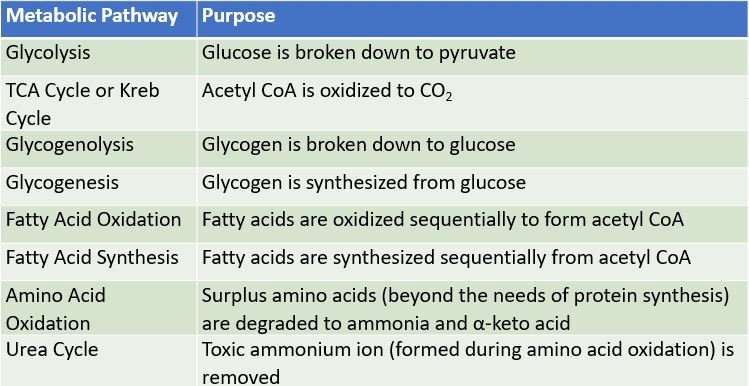
\includegraphics[width=.9\linewidth]{./images/metabolic-pathways.jpg}
\end{center}
\subsubsection{Overall cellular metabolism}
\label{sec:orgdbfec2e}
\begin{center}
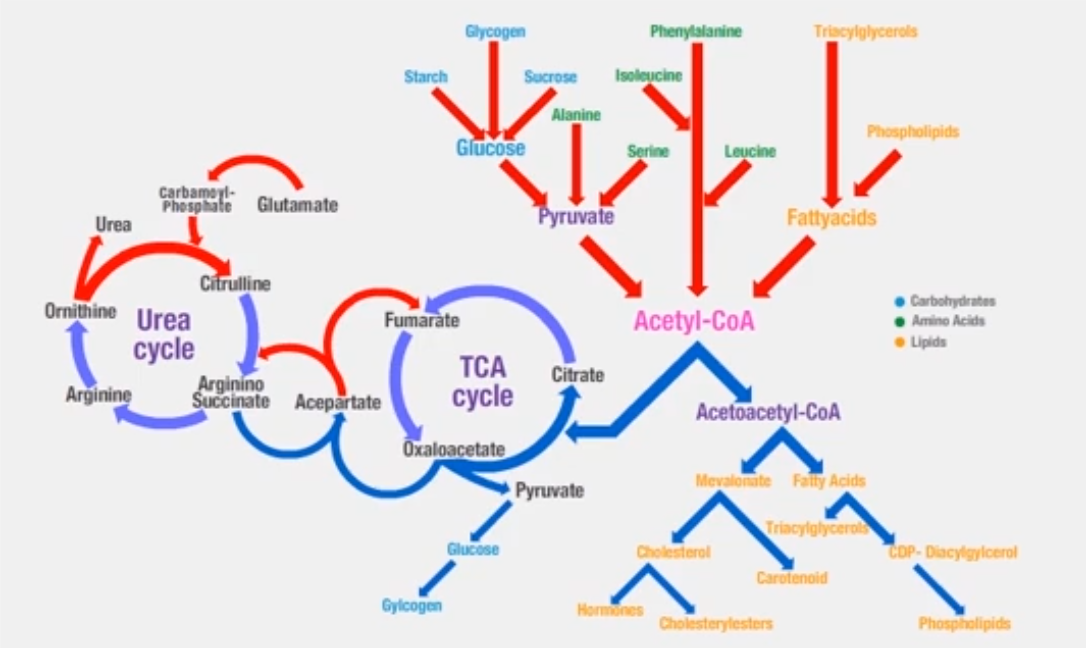
\includegraphics[width=.9\linewidth]{./images/overall-cellular-metabolism.png}
\end{center}

\newpage
\subsubsection{Compartmentalisation of metabolic pathways}
\label{sec:org99abb6e}
In prokaryotes, almost all metabolic pathways occur in the cytoplasm, with some occurring across the cell membrane.


In eukaryotes however, more sophisticated organisation for metabolism can be achieved using organelles such as mitochondrion, chloroplast, endoplasmic reticulum, and nucleus as compartments. This feature of cellular compartmentalisation allows cells to develop strategies of metabolic regular through physical separation accorded by the organelle structures.
\subsection{Cellular respiration}
\label{sec:org9e2c8f9}
Cellular respiration is a metabolic process by which the chemical energy of organic substrates such as glucose is converted into the energy currency of ATP and reducing powers such as NADH, NADPH and \(FADH_2\). It is a universal process occurring both in eukaryotes and in prokaryotes.


Using glucose as the carbohydrate, the process can be summarised as:
\[C_6 H_{12} O_6 + 6O_2 \rightarrow 6CO_2 + 6H_2O + (\text{free energy } + \text{heat})\]

Part of the free energy is coupled to the formation of ATP molecules. Hence, respiration is a catabolic process where glucose is fully oxidised to \(CO_2\) with the liberation and storage of free energy.


Cellular respiration does not occur in one step. It is consists of 3 metabolic pathways occurring in \textbf{4 phases, glycolysis, pyruvate oxidation, tricarboxylic acid (TCA) cycle and electron transfer (transport) chain (ETC) coupled to ATP synthesis}.


In eukaryotic cells, these phases do not occur in one compartment (as they do in prokaryotic cells' cytoplasm) but at three cellular locations, the cytoplasm, the mitochondrial matrix and the inner mitochondrial membrane.

\newpage
\subsection{Glycolysis}
\label{sec:org41e7ab3}
Glycolysis is the metabolic pathway which converts a glucose molecule to 2 pyruvate molecules in the cytoplasm through a series of 10 reactions catalysed by 10 enzymes. Along the way, the two molecules of NAD\(^+\) are reduced to NADH. In addition, two molecules of ADP are phosphorylated to two molecules of ATP. Thus, the net reaction of glycolysis for glucose is:

\begin{equation*}
\begin{gathered}
C_6 H_{12} O_6 + 2ADP + \\
2Pi + 2\text{NAD}^+
\end{gathered}
\rightarrow
\begin{gathered}
2C_3H_4O_3 (\text{Pyruvate}) + 6ATP + \\
2\text{NADH} + 2H^+ + 2H_2O
\end{gathered}
\end{equation*}

\begin{center}
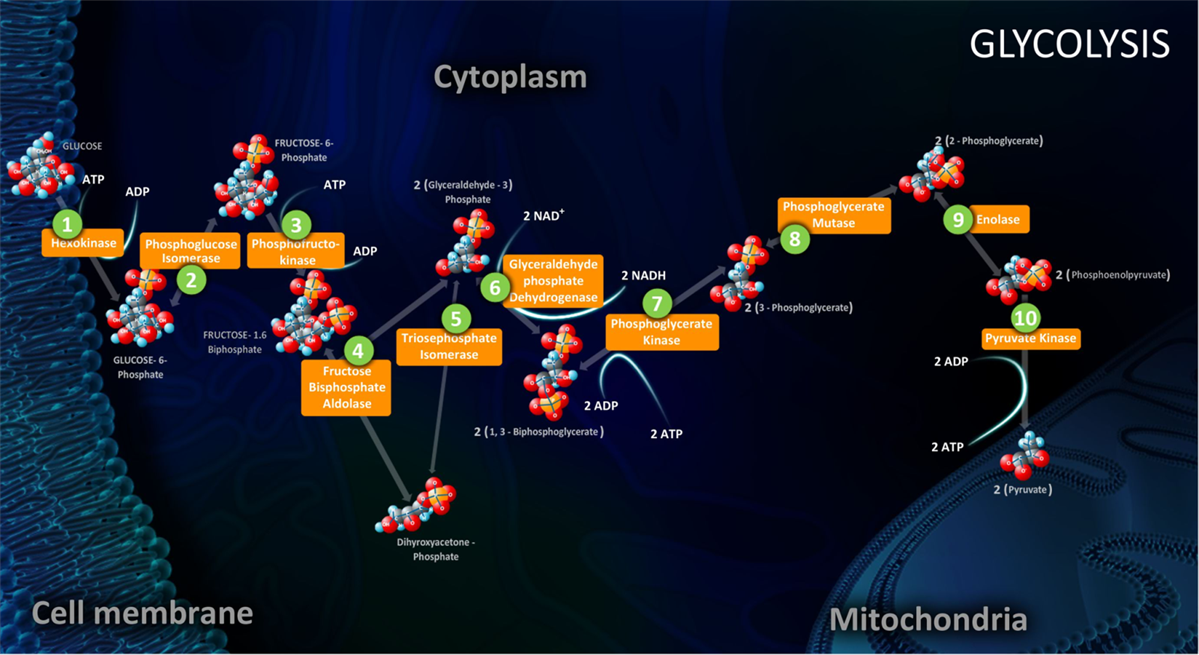
\includegraphics[width=.9\linewidth]{./images/glycolysis.png}
\end{center}

\newpage
\subsection{Pyruvate oxidation}
\label{sec:org318d2e5}
A pyruvate molecule is transported from the cytoplasm to the mitochondrial matrix. There, one of the 3 carbon atoms of pyruvate is cleaved and released as \(CO_2\). The outcome of this reaction is that pyruvate is oxidised by losing two electrons and two protons. NAD+ is reduced, and the remaining acetyl group is attached to CoA, forming acetyl-CoA.
\begin{center}
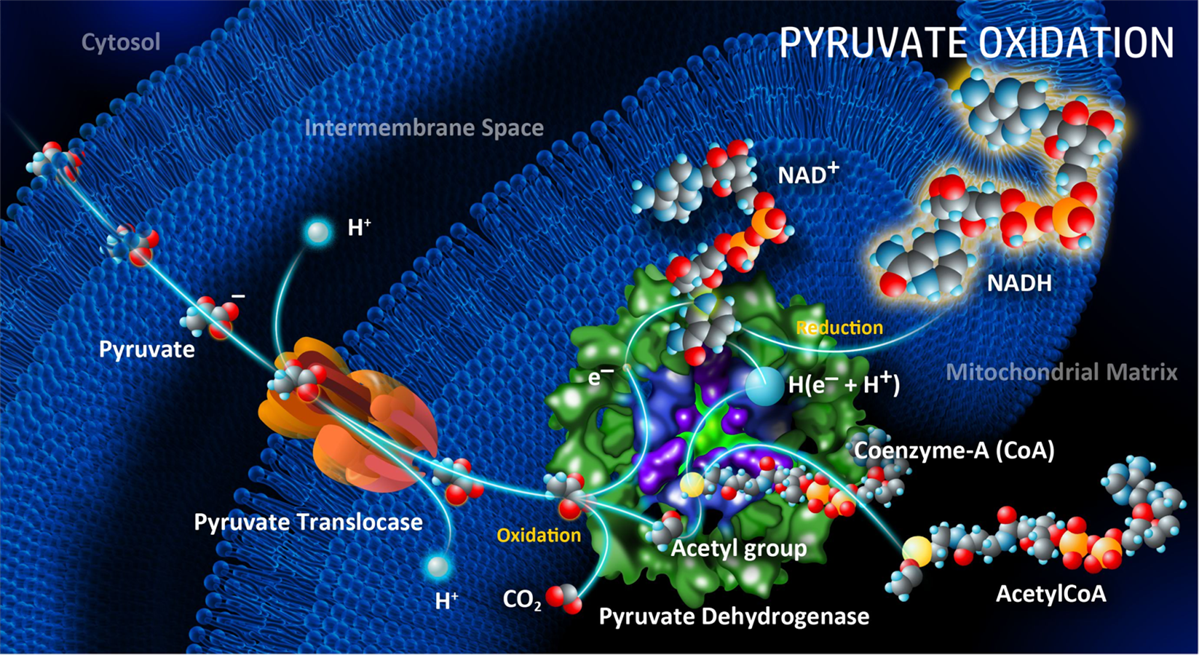
\includegraphics[width=.9\linewidth]{./images/pyruvate-oxidation.png}
\end{center}

\newpage
\subsection{TCA cycle}
\label{sec:org8cece91}
The TCA cycle, also called the citric acid cycle or the Kreb's cycle, is a cyclic pathway that consists of several reaction steps which are mostly oxidative in nature. The cycle occurs in the mitochondrial matrix. The cycle "starts" with the 2-carbon acetyl group of acetyl-CoA combining with a 4 - carbon molecule (oxaloacetic acid, OAA) resulting in a 6 - carbon molecule, citric acid (TCA). The resulting citrate in the first reaction of the cycle undergoes a sequence of oxidative reactions whereby two carbon molecules are oxidised to \(CO_2\) and the OAA molecule is regenerated. This completes on turns of the cycle and allows another turn to start.
\begin{center}
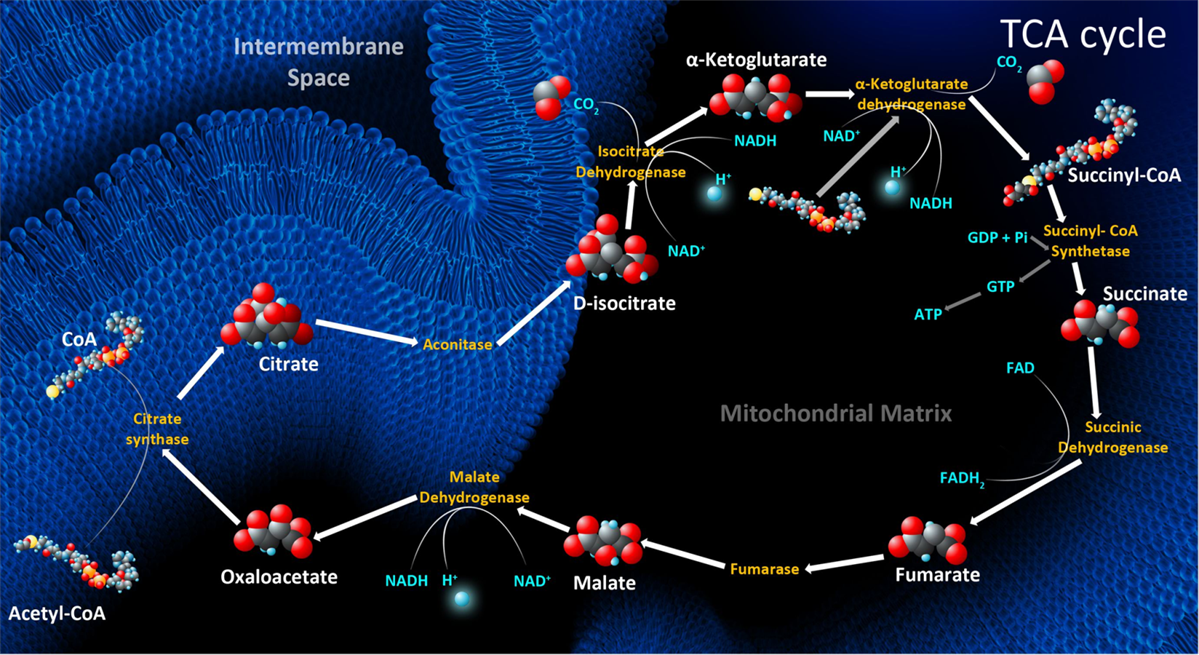
\includegraphics[width=.9\linewidth]{./images/tca-cycle.png}
\end{center}
\subsubsection{Energetics of the TCA cycle}
\label{sec:org5047afb}
Note that both ATP and reducing molecules like NADH and \(FADH_2\) are generated as a result of these 2 turns of TCA.


The inputs and outputs for two turns of the TCA cycle are shown below:
\begin{center}
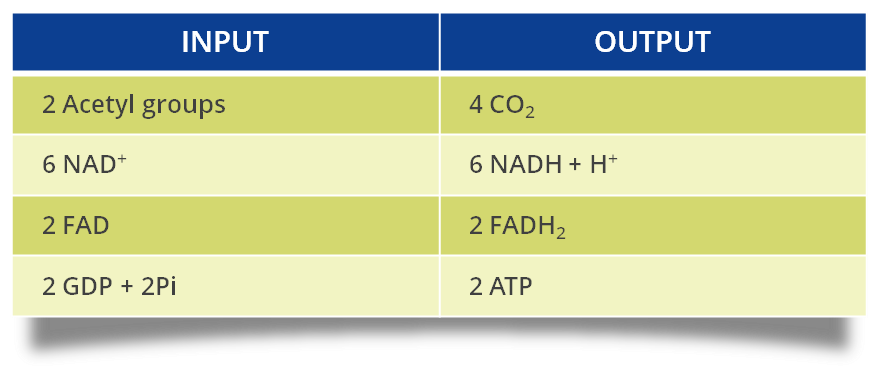
\includegraphics[scale=0.3]{./images/tca-inputs-and-outputs.png}
\end{center}
\subsection{Electron transfer chain (ETC) driven ATP synthesis}
\label{sec:org680c32c}
This is the final phase of cellular respiration, NADH and \(FADH_2\) molecules are oxidised, releasing electrons. The free energy generated from the oxidation of NADH and \(FADH_2\) is used to make more ATP. This phase is divided into three parts: electron transfer chain, formation of proton gradient, and ATP synthesis.
\begin{center}
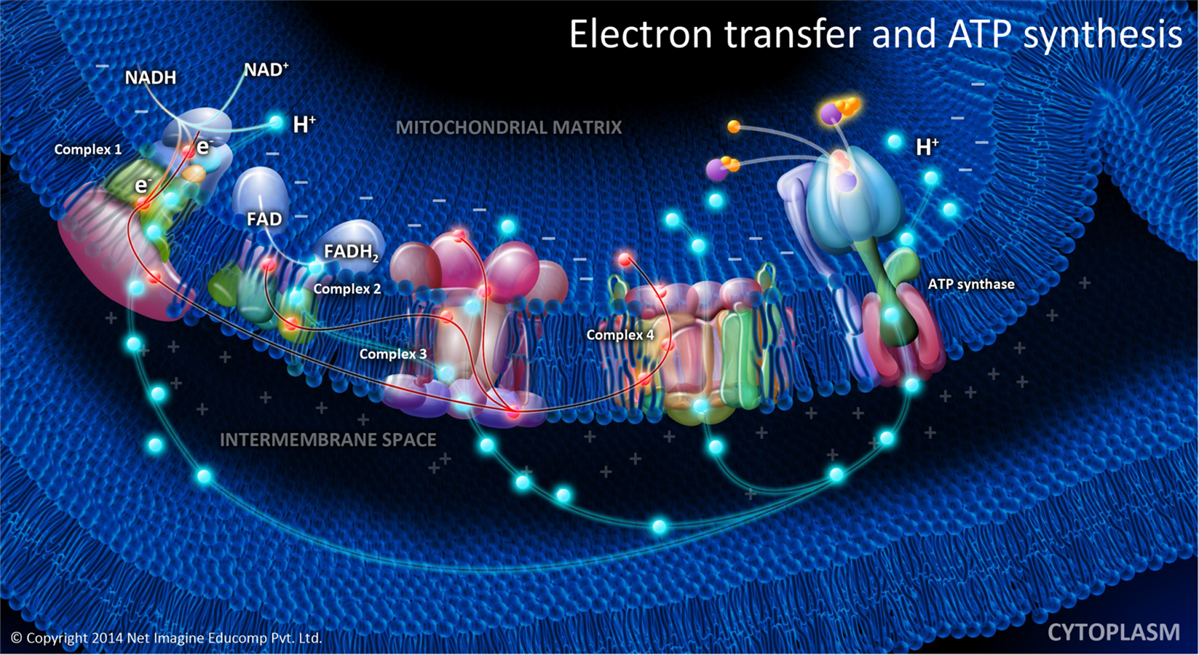
\includegraphics[width=.9\linewidth]{./images/electron-transfer-and-atp-synthesis.png}
\end{center}
\subsubsection{Electron transfer chain (ETC)}
\label{sec:org9f008ae}
The electron transfer chain consists of several electron carriers over which the electrons "hop" through. It starts from NADH and \(FADH_2\) and ends at \(O_2\). In some bacteria and archaea, in the absence of molecular oxygen, different electron acceptors may be used.
\subsubsection{Formation of the proton gradient}
\label{sec:orga42651e}
The electron carriers are localised and embedded in the inner mitochondrial membrane with specific orientations to facilitate electron transfer as well as the formation of the proton gradient. As the electrons pass through the chain, the free energy liberated is used to form a proton gradient across the inner mitochondrial membrane.

\newpage
\subsubsection{ATP synthesis}
\label{sec:orgdd42693}
Any concentration gradient is a potential source of free energy which can be coupled with endergonic processes. In mitochondria, the proton gradient created by the electron transfer chain across its inner membrane is dissipated through a protein complex and the released free energy is captured to synthesise ATP from ADP and Pi. This protein complex is called the ATP synthetase.
\subsection{Autotrophs}
\label{sec:org0031a9d}
Autotrophs just mean that an organism can produce its own food. Autotrophs are able to make use of simple molecules like \(CO_2\) as a carbon source to build complex organic molecules such as polysaccharides and proteins that form the bulk of their body.


Because of this, an autotroph is called a "producer" in the food chain, because this organism "produces" complex organic biomolecules from simple substances present in its surroundings. There are 2 types of autotrophs, photoautotrophs and chemoautotrophs.
\subsection{Photoautotrophs}
\label{sec:orge096a60}
Photoautotrophs use energy from sunlight to produce the energy currency ATP and to convert water (electron source) and carbon dioxide (carbon source) from the air into glucose via a process called photosynthesis. From glucose, other intermediates are further generated for biosynthesis. Examples of photoautotrophs include plants, algae, photosynthetic protists, and cyanobacteria.
\subsection{Chemoautotrophs}
\label{sec:orgcab8b0d}
Chemoautotrophs use energy from chemical compounds to produce ATP and reducing powers, through a process called chemosynthesis. The chemical reactions involve making use of simple inorganic compounds such as \(H_2, H_2 S, NH_3\) and \(Fe^{2+}\) as electron sources, leading to their oxidation. Examples of chemoautotrophs include certain extremophiles such as bacteria and archaea found inside or near active volcanoes, hydrothermal vents in the sea floor and hot water springs.
\subsection{Heterotrophs}
\label{sec:orgccdedae}
Heterotrophs are basically organisms that eat plants or animals for energy. Heterotrophs require more complex organic compounds as the source of carbon. Hence, the lives of heterotrophs are dependent on autotrophs, because these complex substances are made available only through the metabolism of autotrophs.


Therefore, heterotrophs are called "consumers" in the food chain because they live on "producers", which are the autotrophs. There are 2 types of heterotrophs, photoheterortophs and chemoheterotrophs.
\subsection{Photoheterotrophs}
\label{sec:org1186d9f}
Some heterotrophs are versatile enough to use light together with chemical compounds. These heterotrophs use light as an energy source and rely on chemical compounds as electron and carbon sources. Examples of photoheterotrophs are:
\begin{itemize}
\item Purple photosynthetic bacteria. They use light as a source of energy, while using inorganic hydrogen, sulfide or sulfur as electron sources.
\item Pitcher plant. These plants are capable of normal photosynthesis using light, \(CO_2\) and water, and hence are partially photoautotrophs. However, they are also carnivorous, feeding on small insects, hence taking on photoheterotophic metabolism.
\end{itemize}
\subsection{Chemoheterotrophs}
\label{sec:org09ad909}
Chemoheterotrophs make use of chemical compounds for all 3 requirements, which are energy, electrons, and carbon. Examples of chemoheterotrophs are parasites, most bacteria, all fungi, most protozoa, and all animals, which also include humans.
\subsection{Metabolic network}
\label{sec:org6f28a5d}
A metabolic network is the interconnected pathways of biochemical reactions within living cells.

\newpage
\subsection{Metabolic integration (metabolic homeostasis)}
\label{sec:orgf98a7a6}
Metabolic integration is the coordination between different metabolic pathways inside the body and hence metabolic integration is multistep.
\subsubsection{Advantages of metabolic integration}
\label{sec:orgcf22b2b}
\begin{enumerate}
\item Being more energetically efficient. More energy is wasted as heat when a large amount of free energy is released in one single step, compared to when smaller amounts of free energy is being released in a step-wise fashion.
\item Ease of coupling between exergonic and endergonic reactions. With simpler reaction steps, it is more feasible to couple an endergonic reaction to exergonic reactions such as hydrolysis of ATP molecules.
\item Introduction of regulatory mechanisms. Fine-tuning, back-up provision, and coordination with other pathways will be possible with multiple steps of simple reactions, but not if the whole process occurs in one single complex step.
\item Common intermediates allow for metabolic integration. If an intermediate in a particular pathway is also found in other pathways, this intermediate can potentially be made to "multitask" to achieve metabolic integration.
\end{enumerate}

\newpage
\subsubsection{Reduce-reuse-recycle approach}
\label{sec:org79d06c3}
Take the example of the cycling of NADH and NAD\(^+\) in carbohydrate metabolism.


In glycolysis, an NAD\(^+\) molecule is reduced to NADH in one of the reactions. For continues glycolysis, there must be a continuous supple of NAD\(^+\). However, the NAD\(^+\) pool in the cytoplasm is limited. Hence, NADH is re-oxidised via another reaction in the cytoplasm to produce NAD\(^+\) again, essentially "recycling" the NADH.


There are two ways to re-oxidise NADH in the glucose metabolism:
\begin{enumerate}
\item Lactate fermentation
\label{sec:org8c3bffa}

In skeletal muscle cells, NADH is recycled to regenerate NAD\(^+\) through lactate fermentation. Pyruvate (generated during glycolysis) is reduced to lactate in one reaction which oxidises NADH to NAD\(^+\)
\item Alcoholic fermentation
\label{sec:org71ea2e3}

In yeast and some other bacteria, NADH is recycled to regenerate NAD\(^+\) through alcoholic fermentation. Under anaerobic conditions, they reduce pyruvate (generated during glycolysis) to ethanol by oxidising NADH to NAD\(^+\).
\end{enumerate}
\subsubsection{Common intermediates in the reduce-reuse-recycle approach}
\label{sec:orge82c19b}
Pyruvate can be used to generate either lactate of ethanol while recycling NAD\(^+\). It can also be used to synthesise glucose by following a metabolic pathway known as gluconeogenesis. Pyruvate is the common intermediate in the two tracks of metabolic pathways aforementioned. However, the starting molecule for gluconeogenesis need not always by pyruvate. Lactate or amino acids such as alanine can serve as the substrate too. This means that glucose production by gluconeogenesis can be orchestrated by pathways that influence the cellular levels of pyruvate, lactate and amino acids.

\newpage
\subsection{Insulin}
\label{sec:org872854a}
Insulin is a soluble protein that binds to its cell membrane receptor to induce a signal.
\subsection{Homeostasis}
\label{sec:org0cb1b90}
Homeostasis refers to the ability or tendency of an organism to maintain its internal condition fairly stable, i.e, within a range of physiological parameters, such as temperature, blood pressure, pH, as well as the concentrations of blood glucose, other metabolites and ions. When an external event disturbs the balanced state, the organisms counteracts the disturbance by coordinating the functions of all organs and tissues via their metabolic pathways. When the homeostatic mechanism fails due to defective enzymes or extreme environmental fluctuations, disease or disorder sets in.
\subsection{Glucose homeostasis}
\label{sec:org6021b08}
The maintenance of normal glucose level in blood is called glucose homeostasis. Glucose homeostasis strives to maintain the blood glucose concentration at about \(\qty{5}{\unit{mM}}\) (\(\qty{90}{\unit{mg}} / \qty{100}{\unit{ml}}\)) under all conditions. This is especially crucial for our brain, as it uses glucose exclusively as the metabolic fuel, has no fuel storage system, and yet consumes a large amount of energy accounting for at least 20\% of the total energy demand of the body.


If blood glucose falls below a critical level of about \(\qty{2.2}{\unit{mM}}\) (\(\qty{40}{\unit{mg}} / \qty{100}{\unit{ml}}\)), sever and sometimes irreversible damage to brain function may occur. Thus, the first priority of metabolic integration is to maintain glucose homeostasis at any cost with a view to save the brain. Diabetes mellitus is a condition whereby glucose homeostasis is defective.


Glucose metabolism needs to be considered in the context of a fed-starved cycle. The cycle has two stages, the post-absorptive state after a meal of about 2 - 3 hours, and a fasting or starved state after that, before the next meal. The homeostatic responses in each state, involving the hormones insulin and glucagon, lead to the activation and inhibition of the appropriate sets of metabolic pathways that can alter the balance of glucose (the usable form) versus glycogen (the storage form).

\newpage
\subsubsection{Post-absorptive state}
\label{sec:org3641abe}
\begin{enumerate}
\item Soon after a meal that contains carbohydrates as a component, extracellular metabolism works to ensure that glucose from the intestine enters the bloodstream.
\item This results in an increase in the blood glucose level, which is sensed by the pancreas, stimulating it to produce the hormone insulin.
\item Insulin is released into the blood and carried to other organs including its targets: liver, muscle and adipose tissue, where it works to stimulate glucose uptake by the cells, bringing blood glucose concentration down to a normal level.
\item Inside the target cells, metabolic pathways that can decrease cellular glucose concentration by converting glucose to the storage form (glycogen) for future use, are activated.
\end{enumerate}
\subsubsection{Starved or fasting state}
\label{sec:org4111a16}
\begin{enumerate}
\item In this state, even in the absence of visible physical activity, like during sleep, blood glucose is consumed (mainly by the brain) and the level falls below normal.
\item Lowered blood glucose triggers the secretion of glucagon and inhibits insulin release from the pancreas.
\item The main target organ of glucagon is the liver, where glucose production is stimulated. This increases cellular glucose concentration, allowing the liver to export glucose to the blood, restoring glucose level to normal.
\end{enumerate}

\newpage
\subsection{Signal transduction}
\label{sec:orgb5e2bc7}
Signal transduction is a mechanism that transmits the effects of hormones, such as insulin, to target cells. Signal transduction involves a "message" being transmitted from one site (usually remote) to another, most often from the outside to the inside of a cell. It occurs in three steps.
\subsubsection{Reception}
\label{sec:org562240c}
During the reception step, a signal molecule (a messenger) binds to a receptor protein on the target cell's membrane. A part of the receptor molecule protrudes is on the outside of the cell and a part of it is inside the cell.


For example, the hormone insulin is a messenger sent by the pancreas in response to high glucose concentration in bloody. Insulin binds to its specific receptor protein embedded in the plasma membrane of cells of the liver, the muscles and the adipocytes.
\subsubsection{Transduction}
\label{sec:org8fe482f}
During the transduction steps, the part of the receptor molecule inside the cell relays the message to activate the appropriate cellular response.


In the example of insulin, as it binds to the receptor and activates it, certain reactions that produce the second (secondary) messenger molecules are initiated. The second messengers then transmit the signal to the target site by activating a series of reactions sequentially. Cyclic AMP (cAMP) is a common secondary messenger in many signal transduction processes.
\subsubsection{Response}
\label{sec:orgc2325de}
The sequence of reactions initiated through the second messenger eventually reach the end enzyme in this series, which when activated, stimulates or inhibits the target metabolic pathway, which is the intended response. For instance, the transduction process initiated by insulin will eventually reach the regulator that will stimulate consumption of glucose to decrease glucose concentration.

\newpage
\subsubsection{Versatility of the signal transduction system}
\label{sec:org51d5260}
Signal transduction is versatile because of the many ways signal transduction can be configured. The second messengers can be designed to activate not just one series of reactions for targeting one metabolic pathway, but several series of reactions.


For instance, when one insulin binds to its receptor in a liver cell, several metabolic pathways related to the desired response are regulated, like the stimulation of glucose uptake, glycogen synthesis, glycolysis, and fatty acid synthesis.
\subsubsection{Cascade effect}
\label{sec:org1cc9391}
Consider one insulin molecule binding to a receptor and activated 10 second messenger molecules per second. If each second messenger molecule activates 10 enzymes in the cascade per second, 10 messengers will activate 100 enzyme molecules per second.
\section{Energy scheme}
\label{sec:org54f0f10}
Energy \(\rightarrow\) work \(\rightarrow\) system. Whenever some work is done, energy is needed. For example, our body needs energy to do work, and our body gets energy from the food we eat. Another example is that a seed needs energy to sprout, and so the seed gets energy from the chemicals stored inside.

\newpage
\section{Energy change in living systems}
\label{sec:org162b63a}
\begin{enumerate}
\item Most reactions in living things work \textbf{under constant pressure}.
\item Most processes occur in solid and liquid phases, which are mostly \textbf{constant in volume}. Even the occasional by-products of gases end up being dissolved in liquids.
\end{enumerate}

Since \(W\) is affected by changes in pressure and volume and those are constant in living systems:
\[\Delta E = q\]

Under such conditions:
\begin{itemize}
\item \(\Delta E\) is referred to as the enthalpy of a system, or \(\Delta E = \Delta H\)
\item Due to this relationship, the term enthalpy often appears when heat exchange is described in biological reactions.
\end{itemize}
\section{Adenosine triphosphate (ATP) as energy}
\label{sec:orgfc6b4ee}
\begin{itemize}
\item ATP hydrolysis is a common exergonic reaction which is coupled to many endergonic reactions of metabolic pathways.
\item Various activities in a cell are nearly always powered by the hydrolysis of ATP.
\item ATP is a renewable resource that can be regenerated by the addition of a phosphate group to ADP (which is powered by exergonic reactions during cellular respiration).
\item The turnover of ATP is very high in living organisms. A resting human adult consumes roughly \(\qty{40}{\unit{kg}}\) of ATP per day and a working muscle cell recycles its entire pool of ATP once each minute. More than 10 million ATP molecules are consumed and regenerated per second per cell.
\end{itemize}

\newpage
\section{Extracellular metabolism}
\label{sec:org42fa75e}

\subsection{Carbohydrates}
\label{sec:org393d963}
\begin{itemize}
\item Starch is the major carbohydrate in our food. Other carbohydrates that can be found in foodstuff are sucrose, lactose and sometimes maltose.
\item Starch digestion is started in the mouth by the enzyme amylase, which is secreted by the salivary glands and continues in the upper part of the stomach.
\item Starch, sucrose, lactose, and maltose are then fully digested to monosaccharides (glucose, galactose and fructose) in the small intestine by pancreatic amylase.
\item The monosaccharides need to be absorbed "into the body" across the epithelial cells lining the villus.
\item Fructose enters the epithelial cells by facilitated diffusion, while glucose and galactose enter by active transport.
\item They then move through the epithelial cells and cross the membrane by facilitated diffusion in order to enter the blood.
\item They are then distributed to and taken up by cells, within which cellular metabolism occurs.
\end{itemize}

\newpage
\subsection{Proteins}
\label{sec:orgd47c141}
\begin{itemize}
\item The extracellular metabolism of proteins beings in the stomach.
\item In the acidic pH of the stomach, the dietary proteins are first unfolded (denatured).
\item The enzyme pepsin then cleaves some peptide bonds in these unfolded proteins, thereby making small peptides.
\item These small peptides are then carried to the small intestine where the pH is near neutral. The peptides cannot refold since they are only fragments of the original proteins.
\item In the small intestine, the peptides are further cut by other enzymes, such as trypsin, into amino acids and smaller peptides.
\item They are now ready to be transported across the epithelial cells of the intestine to the inside of the body. Similar to the monosaccharides, amino acids cross the epithelial cell membranes into the capillaries to enter the blood, and get circulated to be taken up by cells to enter the cellular metabolism phase.
\end{itemize}

\newpage
\subsection{Fats (triglycerides)}
\label{sec:org83e954c}
\begin{itemize}
\item Fats are insoluble in the aqueous medium such as the cytosol or blood.
\item Thus, fats in our food first aggregate into large droplets through hydrophobic interaction in the upper part of the stomach and move to the intestine.
\item Here, these large lipid droplets are emulsified into smaller droplets by bile salt and phospholipids which have been secreted into the small intestine by the liver (stored in the gall bladder).
\item Emulsified droplets of fat are then digested by the enzyme lipase, secreted by the pancreas, into fatty acids and monoglycerides.
\item The fatty acids and monoglycerides then diffuse into the intestinal epithelial cells, where they are recombined by enzymes into triglycerides again.
\item These triglycerides aggregate and are released as chylomicrons through the other side of the epithelial cells via exocytosis.
\item Chylomicrons find their way into the lymphatic system and are then delivered to the systemic veins to enter the circulation for eventual uptake by the liver, to be broken down into fatty acids again.
\end{itemize}

\newpage
\section{Large amount of water is needed to digest food}
\label{sec:orgc2441c4}
\begin{itemize}
\item For an average adult, over 8 litres of water enters the GI tract to digest less than \(\qty{1}{\unit{kg}}\) for foodstuff.
\item Of this 8 litres of water, 99\% is absorbed back into the blood at the end of the process.
\end{itemize}

The reason for requiring is due to water being needed to hydrolyse the macromolecules into their monomeric units (monosaccharides, amino acids, nucleotides and fatty acids).

\begin{figure}[htbp]
\centering
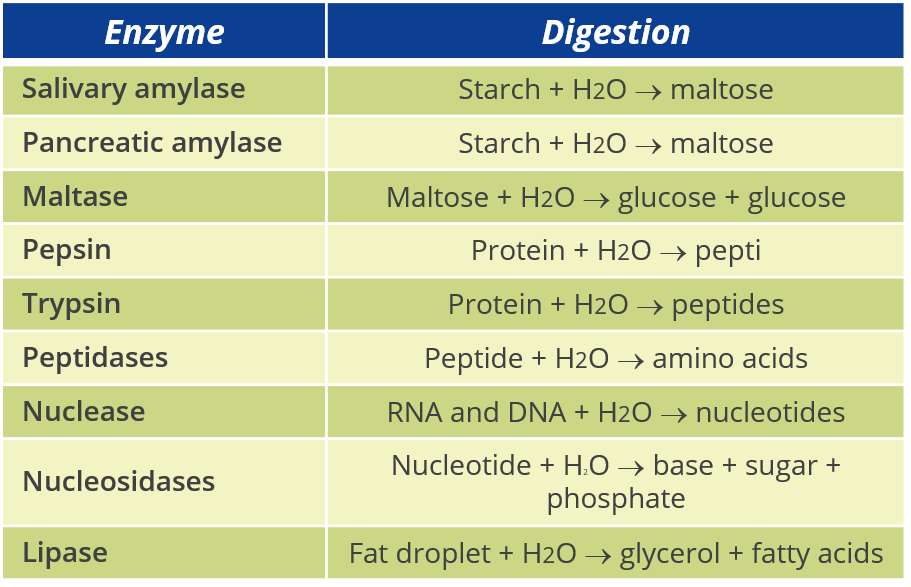
\includegraphics[width=.9\linewidth]{./images/hydrolysis-table.png}
\caption{Water is used for the hydrolysis of most macromolecules.}
\end{figure}

\newpage
\subsection{Water in digestion}
\label{sec:orgd11de9f}

\begin{figure}[htbp]
\centering
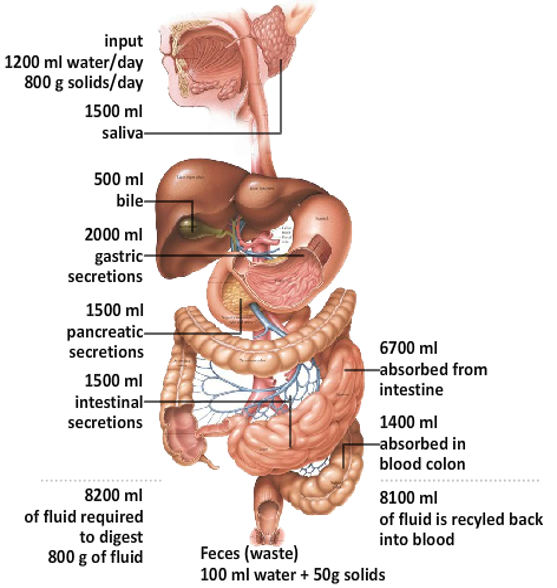
\includegraphics[width=.9\linewidth]{./images/water-during-digestion.png}
\caption{The amount of water used or absorbed in the body during digestion.}
\end{figure}

\newpage
\section{Metabolic fates of pyruvate}
\label{sec:org43384f9}
Pyruvate can be channelled to one of the 4 options of metabolism below:
\subsection{Pyruvate oxidation}
\label{sec:orgc25ead4}
Pyruvate forms acetyl CoA. This happens in plants, animals, and bacteria, under aerobic conditions.
\subsection{Lactate fermentation}
\label{sec:orge5dc811}
Pyruvate forms lactate. This happens in red blood cells, highly active muscles, and bacteria under oxygen limiting (anaerobic) conditions.
\subsection{Ethanol fermentation}
\label{sec:orge9f9b8a}
Pyruvate forms ethanol. This happens in yeast and some bacteria under anaerobic conditions.
\subsection{Gluconeogenesis}
\label{sec:org76916af}
Pyruvate goes into an anabolic pathway to form back glucose.
\section{Specifying a metabolic type}
\label{sec:org2d6cb89}
There are 3 primary requirements that need to be examined when considering the metabolic type of an organism.
\begin{enumerate}
\item Energy source
\label{sec:org6313433}

The energy source is form of energy that gets transferred from the environment into the organism.
\item Electron source
\label{sec:org6308bc1}

Electron source is compound used by the organism to ultimately generate its reducing powers (reductants), such as NADH and \(FADH_2\).
\item Carbon source
\label{sec:orgf982c81}

The carbon source is used to build up the physical body.
\end{enumerate}
\subsection{Animal example}
\label{sec:orgbdf7394}
In animals, organic material such as carbohydrates can be the source of all 3 requirements, achieved through the overall reaction shown below:
\[CH_2 O (\text{carbohydrates}) + O_2 \rightarrow CO_2 + H_2 O\]

As seen in the process of cellular respiration, the organic material carbohydrates satisfy all three requirements in the following ways:
\subsubsection{Energy source}
\label{sec:org57caba5}
The energy source is chemical potential energy. The oxidation of carbohydrates generates energy as ATP.
\subsubsection{Electron source}
\label{sec:orgc3d128d}
The oxidation of carbohydrates produce reducing powers in the form of NADH and \(FADH_2\).
\subsubsection{Carbon source}
\label{sec:org7e7c2a9}
The breakdown of carbohydrates to smaller units generates a pool of carbon sources that can be drawn upon to make metabolic intermediates and various biomolecules.
\subsection{Plant example}
\label{sec:orge874d85}
In photosynthetic organisms, the three requirements are coming from different sources. In green plants, for example, the requirements are satisfied by having light, water and carbon dioxide, achieved through the overall reaction shown below:
\[CO_2 + H_2 O (\text{in the presence of light}) \rightarrow CH_2 O (\text{carbohydrates}) + O_2\]
\subsubsection{Energy source}
\label{sec:org1cd8aae}
The energy source is light. The source of energy that oxidises water to generate energy as ATP and also fix \(CO_2\) is light.
\subsubsection{Electron source}
\label{sec:org21991ea}
\(H_2 O\) is the source of electrons needed to produce NADPH, which is the reducing power found primarily in plants.
\subsubsection{Carbon source}
\label{sec:org3820818}
\(CO_2\) is fixed into organic compounds to become metabolic intermediates for making various biomolecules of the plant body.
\section{Metabolic division of labour among organs}
\label{sec:org1b6985b}
Each organ has its own metabolic profile specified by its function:
\begin{itemize}
\item Skeletal muscle performs motion
\item Adipose tissue stores and releases fats
\item The brain pumps ions to produce electrical signals and synthesise neurotransmitters
\item The liver plays a central role by performing functions as the "watch dog" of all the other organs.
\end{itemize}

Each organ is specialised in terms of the metabolic fuel used, the type of fuel stored, and the metabolic fuel available to transport to other organs. Let's take the example of glucose metabolism.


\begin{enumerate}
\item During prolonged movement, skeletal muscle cells utilise glucose (by initiating glycolysis) to produce energy for muscular action, and produce excess lactate (from pyruvate, generated during glycolysis) as a result.
\item The lactate from muscles is then transported via blood circulation to the liver. Here, lactate is converted to glucose by gluconeogenesis, a metabolic pathway not present in muscle cells.
\item This pool of "new" glucose produced by the liver is then transported to muscles here it can be used to further generate energy to sustain more muscular activities.
\end{enumerate}

The above is a metabolic division of labour between skeletal muscles and the liver. The skeletal muscles specialise in using glucose, whereas the liver takes care of the recycling of glucose from lactate produced by the muscles.
\end{document}
